\chapter{Scalable Runtime Remote Attestation for Complex Systems} % 
%Main chapter title
\label{chp:runtime-protection-untrusted} 

%After protecting the untrusted code in~\ref{chp:static-protection}, I will 
%focus on runtime attacks (code-reuse attacks) against the untrusted code.
%
%The answer to this question is addressed in this paper:
%\begin{itemize}
%	\item ScaRR: Scalable Runtime Remote Attestation for Complex Systems (RAID 
%	2019).
%\end{itemize}

%\section{Introduction}
%\label{sec:introduction}

%\todo{define what we mean for complex systems!!!}

%RA is a procedure that allows an entity (\ie the \emph{Verifier}) 
%to verify the status of a device (\ie the \emph{Prover}) from a remote 
%location. This is achieved by having first the \emph{Verifier} sending a 
%challenge to the \emph{Prover}, which replies with a report. 
%Then, the \emph{Verifier} analyzes the report to identify whether the 
%\emph{Prover} has been compromised~\cite{anati2013innovative}. 
%In standard RA, usually defined as static, the \emph{Prover} verification 
%involves the integrity of specific hardware and software properties (\eg the 
%\emph{Prover} has loaded the correct software).
%On the market, there are already several available products implementing 
%static 
%RA, such as Software Guard Extensions (SGX)~\cite{costan2016intel} or Trusted 
%Platform Module (TPM)~\cite{tomlinson2017introduction}.
%However, these do not provide a defence against runtime attacks (\eg the 
%control-flow ones)
%that aim to modify the program runtime behaviour. 
%Therefore, to identify \emph{Prover} runtime modifications, researchers 
%proposed runtime RA. Among the different solutions belonging to this category, 
%there are also the control-flow attestation approaches, which
%encode the information about the executed control-flow of a 
%process~\cite{abera2016c,aberadiat}.
%
%In comparison to static RA, the runtime one is relatively new, and today there 
%are no reliable products available on the market since researchers have mainly 
%investigated runtime RA for embedded 
%devices~\cite{abera2016c,zeitouni2017atrium,aberadiat,dessouky2017fat,Dessouky:2018:LLH:3240765.3240821}:
%most of them encode the complete execution path of a \emph{Prover} in a single 
%hash~\cite{abera2016c,zeitouni2017atrium,dessouky2017fat}; 
%some~\cite{aberadiat} compress it in a simpler representation and rely on a 
%policy-based verification schema; 
%other ones~\cite{Dessouky:2018:LLH:3240765.3240821} adopt symbolic execution 
%to 
%verify the control-flow information continuously sent by the \emph{Prover}. 
%Even if they have different performances, none of the previous solutions can 
%be 
%applied to a complex system (\eg virtual machines in a cloud) due to the 
%following reasons: 
%\begin{enumerate*}[label=(\roman*)]
%	\item representing all the valid execution paths through hash values is 
%	unfeasible (\eg the number of execution paths tends to grow exponentially 
%	with the size of the program),
%	\item the policy-based approaches might not cover all the possible attacks,
%	\item symbolic execution slows down the verification phase.
%\end{enumerate*}

In this chapter, we propose ScaRR, the first runtime RA schema for complex 
systems.
In particular, we focus on environments such as Amazon Web Services (\cite{aws})
or Microsoft Azure (\cite{azure}). 
Since we target such systems, we require support for features such as 
multi-threading.
Thus, ScaRR provides the following achievements with respect to the current 
solutions supporting runtime RA: 
\begin{enumerate*}[label=(\roman*)]
	\item it makes the runtime RA feasible for any software,
	\item it enables the \emph{Verifier} to verify intermediate states of the 
	\emph{Prover} without interrupting its execution,
	\item it supports a more fine-grained analysis of the execution path where 
	the attack has been performed. 
\end{enumerate*}
We achieve these goals thanks to a novel model for representing the execution 
paths of a program, which is based on the fragmentation of the whole path into 
meaningful sub-paths. As a consequence, the \emph{Prover} can send a series of 
intermediate partial reports, which are immediately validated by the 
\emph{Verifier} thanks to the lightweight verification procedures performed.  

ScaRR is designed to defend a \emph{Prover}, equipped with a trusted anchor and 
with a set of the standard solutions (\eg 
W$\oplus$X/DEP~\cite{pinzari2003introduction},
Address Space Layout Randomization - ASLR~\cite{kil2006address}, and Stack 
Canaries~\cite{baratloo2000transparent}), from attacks performed in the 
user-space and aimed at modifying the \emph{Prover} runtime behaviour. The 
current implementation of ScaRR requires the program source code to be properly 
instrumented through a compiler based on LLVM~\cite{lattner2004llvm}. However, 
it is possible to use lifting techniques~\cite{mcsema}, as well. 
Once deployed, ScaRR allows to verify on average $2M$ control-flow events per 
second, which is significantly more than the few hundred 
per second~\cite{Dessouky:2018:LLH:3240765.3240821} or the thousands per 
second~\cite{aberadiat} verifiable through the existing solutions.

\textbf{Contribution.} The contributions of this work are the following ones: 
\begin{itemize}
	\item We designed a new model for representing the execution path for 
	applications of any complexity.% together with a fine-grained detection of 
	%runtime errors location in the program;
	%\item We describe and analyze a runtime RA schema suitable for complex 
	%systems in cloud environments.
	\item We designed and developed ScaRR, the first schema that supports 
	runtime RA for complex systems.
	\item We evaluated the ScaRR performances in terms of: 
	\begin{enumerate*}[label=(\roman*)]
		\item attestation speed (\ie the time required by the \emph{Prover} to 
		generate a partial report),
		\item verification speed (\ie the time required by the \emph{Verifier} 
		to evaluate a partial report),
		\item overall generated network traffic (\ie the network traffic 
		generated during the communication between \emph{Prover} and 
		\emph{Verifier}).
	\end{enumerate*}
\end{itemize}

\section{Threat Model and Requirements}
\label{sec:threat-model}

In this section, we describe the features of the \emph{Attacker} and the 
\emph{Prover} involved in our threat model. Our assumptions are in line with 
other RA 
schemes~\cite{costan2016intel,winter2008trusted,abera2016c,aberadiat,Dessouky:2018:LLH:3240765.3240821}.

\paragraph{Attacker.}
We assume to have an attacker that aims to control a remote service, such as a 
Web Server or a Database Management System (DBMS), and that has already 
bypassed the default protections, such as Control Flow Integrity (CFI). To 
achieve his aim, the attacker can adopt different techniques, among which: 
Return-Oriented Programming (ROP)/ Jump-Oriented Programming (JOP) 
attacks~\cite{carlini2014rop,bletsch2011jump}, function hooks~\cite{7778160}, 
injection of a malware into the victim process, installation of a data-only 
malware in user-space~\cite{vogl2014persistent}, or manipulation of other 
user-space processes, such as security monitors. 
In our threat model, we do not consider physical attacks (our complex systems
are supposed to be virtual machines), pure data-oriented attacks (\eg attacks
that do not alter the original program CFG), self-modifying code, and dynamic 
loading of code at runtime (\eg just-in-time 
compilers~\cite{suganuma2000overview}).
We refer to Section~\ref{ssec:security+privacy+consideration} for a 
comprehensive
attacker analysis.

\paragraph{Prover.}
The \emph{Prover} is assumed to be equipped with:
\begin{enumerate*}[label=(\roman*)]
	%	\item a trusted anchor,
	\item a trusted anchor that guarantees a static RA,
	\item standard defence mitigation techniques, such as W$\oplus$X/DEP, ASLR.
\end{enumerate*}
In our implementation, we use the kernel as a trusted anchor, which is a 
reasonable assumption if the machines have trusted modules such as a 
TPM~\cite{tomlinson2017introduction}. 
However, we can also use a dedicated hardware, as discussed in 
Section~\ref{sec:discussion}. The \emph{Prover} maintains sensitive information 
(\ie shared keys and cryptographic functions) in the trusted anchor and uses it 
to generate fresh reports, that cannot be tampered by the attacker. 

\section{ScaRR Control-Flow Model}
\label{sec:model}

ScaRR is the first schema that allows to apply runtime RA on complex systems. 
To achieve this goal, it relies on a new model for representing the 
CFG/execution path of a program. In this section, we illustrate first the main 
components of our control-flow model (Section~\ref{ssec:basic_concepts}) and, 
then, the challenges we faced during its design (Section~\ref{ssec:challenges}).

\subsection{Basic Concepts}
\label{ssec:basic_concepts}

The ScaRR control-flow model handles BBLs at assembly level and involves two 
components: \emph{checkpoints} and \emph{List of Actions (LoA)}.


A \emph{checkpoint} is a special BBL used as a delimiter for identifying the 
start or the end of a sub-path within the CGF/execution path of a program. A 
\emph{checkpoint} can be: \emph{thread beginning/end}, if it identifies the 
beginning/end of a thread; \emph{exit-point}, if it represents an exit-point 
from an application module (\eg a system call or a library function 
invocation); \emph{virtual-checkpoint}, if it is used for managing special 
cases such as \emph{loops} and \emph{recursions}. 

A \emph{LoA} is the series of significant edges that a process traverses to 
move from a \emph{checkpoint} to the next one. Each edge is represented through 
its source and destination BBL and, comprehensively, a \emph{LoA} is defined 
through the following notation:
$$
[(\text{BBL}_{s1},\text{BBL}_{d1}), \dots, (\text{BBL}_{sn},\text{BBL}_{dn})].
$$
Among all the edges involved in the complete representation of a CFG, we 
consider only a subset of them.
In particular, we look only at those edges that identify a unique execution 
path: procedure call, procedure return and branch (\ie conditional and indirect 
jumps). 

To better illustrate the ScaRR control-flow model, we now recall the example 
introduced in Section~\ref{sec:background}. 
Among the six nodes belonging to the CFG of the example, only the following 
four ones are \emph{checkpoints}: $N_1$, since it is a \emph{thread beginning}; 
$N_3$ and $N_4$, because they are \emph{exit-points}, and $N_6$, since it is a 
\emph{thread end}. In addition, the \emph{LoAs} associated to the example are 
the following ones:  
\begin{equation*}
\begin{split}
N_1-N_3 &\Rightarrow [(N_2, N_3)] \\    
N_1-N_4 &\Rightarrow [(N_2, N_4)] \\ 
N_3-N_6 &\Rightarrow [] \\
N_4-N_6 &\Rightarrow [].
\end{split}
\end{equation*}
On the left we indicate a pair of \emph{checkpoints} (\eg $N_1-N_3$), while on 
the right the associated \emph{LoA} (empty \emph{LoAs} are considered valid).

\subsection{Challenges}
\label{ssec:challenges}
\emph{Loops}, \emph{recursions}, \emph{signals}, and \emph{exceptions} involved 
in the execution of a program introduce new challenges in the representation of 
a CFG since they can generate uncountable executions paths. For example, 
\emph{loops} and \emph{recursions} can generate an indefinite number of 
possible combinations of \emph{LoA}, while \emph{signals}, as well as 
\emph{exceptions}, can introduce an unpredictable execution path at any time.

\textbf{Loops.}
In Figure~\ref{fig:challenge-III}, we illustrate the approach used to handle 
\emph{loops}.
\begin{figure}[t]
	\centering
	\begin{subfigure}[t]{0.4\textwidth}
		\centering
		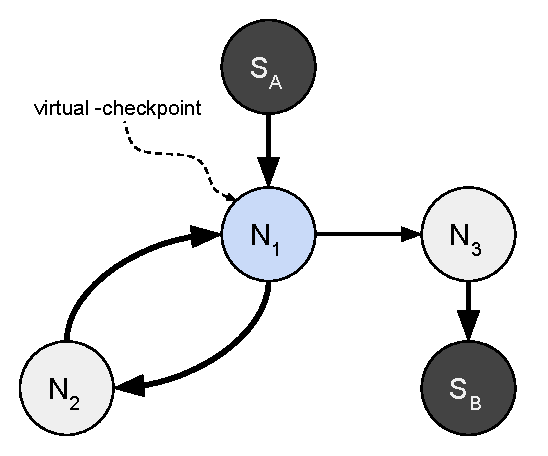
\includegraphics[width=0.8\textwidth]{fig_c4/challenge-III.pdf}
		\caption{Loop example in the ScaRR control-flow model.}
		\label{fig:challenge-III}
	\end{subfigure}
	\hfill
	\begin{subfigure}[t]{0.5\textwidth}
		\centering
		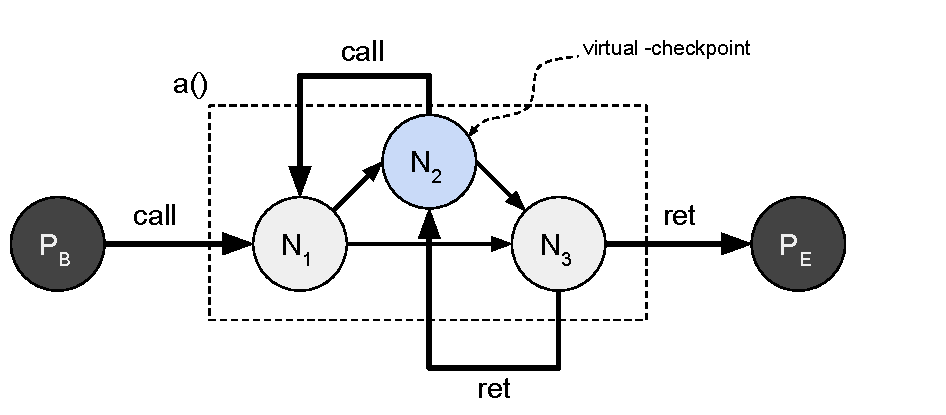
\includegraphics[width=\textwidth]{fig_c4/challenge-IV.pdf}
		\caption{Recursion example in the ScaRR control-flow model.}
		\label{fig:challenge-IV}
	\end{subfigure}
	\label{fig:challenges}
	\caption{ScaRR model challenges.}
\end{figure}
Since it is not always possible to count the number of iterations of a loop, we 
consider the conditional node of the \emph{loop} (\texttt{$N_1$}) as a 
\emph{virtual-checkpoint}. 
Thus, the \emph{LoAs} associated to the example shown in 
Figure~\ref{fig:challenge-III} are as follows: 
\begin{equation*}
\begin{split}
S_A-N_1 &\Rightarrow [] \\    
N_1-N_1 &\Rightarrow [(N_1, N_2)] \\ 
N_1-S_B &\Rightarrow [(N_1, N_3)].
\end{split}
\end{equation*}

\textbf{Recursions.}
In Figure~\ref{fig:challenge-IV}, we illustrate our approach to handle 
\emph{recursions},
\ie a function that invokes itself. 
%
Intuitively, the \emph{LoAs} connecting \texttt{$P_B$} and \texttt{$P_E$} 
should contain all the possible invocations made by \texttt{a()} towards 
itself, but the number of invocations is indefinite. Thus, we consider the node 
performing the recursion as a \emph{virtual-checkpoint} and model only the path 
that could be chosen, without referring to the number of times it is really 
undertaken. The resulting \emph{LoAs} for the example in 
Figuree~\ref{fig:challenge-IV} are the following ones: 
\begin{equation*}
\begin{split}
P_B-N_2 &\Rightarrow [(P_B, N_1),(N_1,N_2)] \\    
N_2-N_2 &\Rightarrow [(N_2, N_1),(N_1,N_2)] \\ 
N_2-N_2 &\Rightarrow [(N_2, N_1),(N_1, N_3),(N_3, N_2)] \\
N_2-P_E &\Rightarrow [(N_2, N_1),(N_1, N_3),(N_3, P_E)] \\
P_B-P_E &\Rightarrow [(P_B, N_1),(N_1, N_3),(N_3, P_E)].
\end{split}
\end{equation*}

Finally, the \emph{virtual-checkpoint} can be used as a general approach to 
solve every situation in which an indirect jump targets a node already present 
in the \emph{LoA}.

\textbf{Signals.}
When a thread receives a \emph{signal}, its execution is stopped and, after a 
context-switch, it is diverted to a dedicated handler (\eg a function).
This scenario makes the control-flow unpredictable, since an interruption can 
occur at any point during the execution. To manage this case, ScaRR models the 
signal handler as a separate thread (adding \emph{beginning/end thread 
checkpoints})
and computes the relative \emph{LoAs}. If no handler is available for the 
\emph{signal} that interrupted the program, the entire process ends 
immediately, producing a wrong \emph{LoA}. 

\textbf{Exception Handler.}
Similar to \emph{signals}, when a thread rises an \emph{exception}, the 
execution path is stopped
and control is transferred to a catch block. 
Since ScaRR has been implemented for Linux,
we model the catch blocks as a separate thread (adding \emph{beginning/end 
thread checkpoints}),
but it is also possible to adapt ScaRR to fulfill different exception handling 
mechanisms (\eg in Windows).
In case no catch block is suitable for the \emph{exception} that was thrown, 
the process gets interrupted and the generated \emph{LoA} is wrong.


%\section{System Overview}
\section{System Design}
\label{sec:proposal}

To apply runtime RA on a complex system, there are two fundamental 
requirements: 
\begin{enumerate*}[label=(\roman*)]
	\item handling the representation of a complex CFG or execution path,
	\item having a fast verification process.
\end{enumerate*}
Previous works have tried to achieve the first requirement through different 
approaches. A first 
solution~\cite{abera2016c,zeitouni2017atrium,dessouky2017fat} is based on the 
association of all the valid execution paths of the \emph{Prover} with a single 
hash value. 
Intuitively, this is not a scalable approach because it does not allow to 
handle complex CFG/execution paths. 
On the contrary, a second approach~\cite{Dessouky:2018:LLH:3240765.3240821} 
relies on the transmission of all the control-flow events to the 
\emph{Verifier}, 
which then applies a symbolic execution to validate their correctness. While 
addressing the first requirement, this solution suffers from a slow 
verification phase, which leads toward a failure in satisfying the second 
requirement. 

Thanks to its novel control-flow model, ScaRR enables runtime RA for complex 
systems, since its design specifically considers the above-mentioned 
requirements with the purpose of addressing both of them. In this section, we 
provide an overview of the ScaRR schema (Section~\ref{ssec:scarr_overview}) 
together with the details of its workflow (Section~\ref{ssec:scarr_details}), 
explicitly motivating how we address both the requirements needed to apply 
runtime RA on complex systems. 

\subsection{Overview}
\label{ssec:scarr_overview}
Even if the ScaRR control-flow model is composed of \emph{checkpoints} and 
\emph{LoAs}, the ScaRR schema relies on a different type of elements, which are 
the \emph{measurements}. Those are a combination of \emph{checkpoints} and 
\emph{LoAs} and contain the necessary information to perform runtime RA. 
Figure~\ref{fig:overview} shows an overview of ScaRR, which encompasses the 
following four components: a \emph{Measurements Generator}, for identifying all 
the program valid \emph{measurements}; 
a \emph{Measurements DB}, for saving all the program valid \emph{measurements};
a \emph{Prover}, which is the machine running the monitored program;
a \emph{Verifier}, which is the machine performing the program runtime 
verification. 

\begin{figure*}[h]
	\centering
	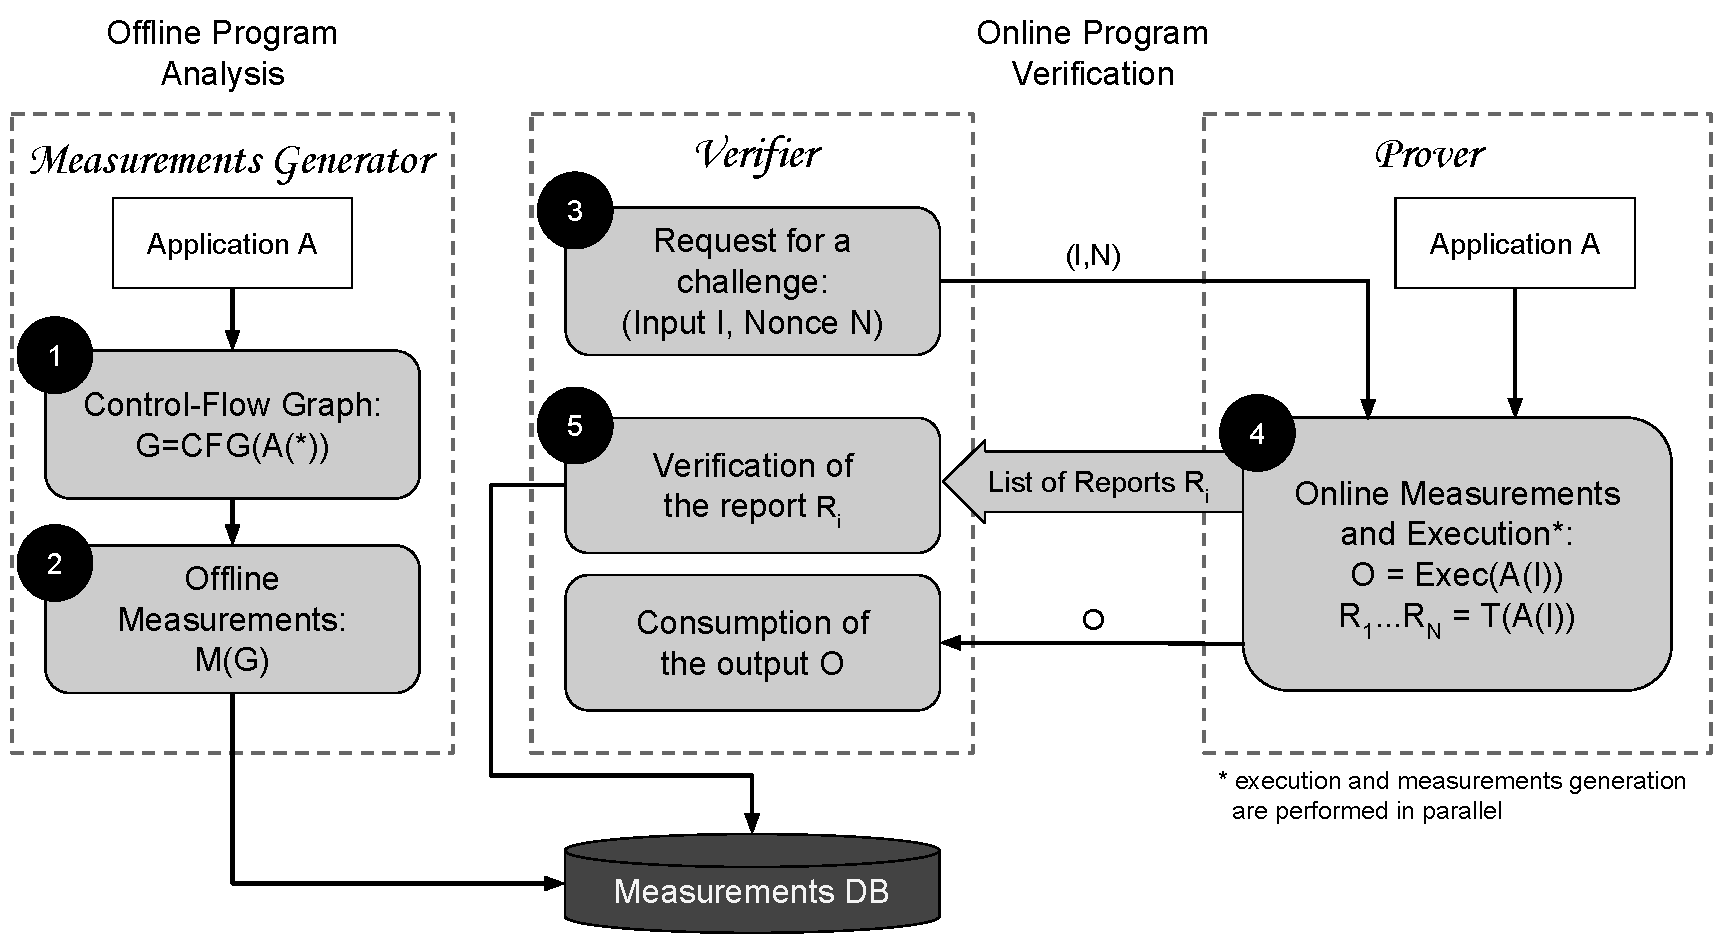
\includegraphics[width=0.8\textwidth]{fig_c4/overview.pdf}
	\caption{ScaRR system overview.}
	\label{fig:overview}
\end{figure*}

As a whole, the workflow of ScaRR involves two separate phases: an 
\emph{Offline Program Analysis} and an \emph{Online Program Verification}. 
During the first phase, the \emph{Measurements Generator} calculates the CFG of 
the monitored \emph{Application A} (Step 1 in Figure~\ref{fig:overview}) and, 
after generating all the \emph{Application A} valid \emph{measurements}, it 
saves them in the \emph{Measurements DB} (Step 2 in Figure~\ref{fig:overview}).
During the second phase, the \emph{Verifier} sends a challenge to the 
\emph{Prover} (Step 3 in Figure~\ref{fig:overview}).
Thus, the \emph{Prover} starts executing the  \emph{Application A} and sending 
partial reports to the \emph{Verifier} (Step 4 in Figure~\ref{fig:overview}). 
The \emph{Verifier} validates the freshness and correctness of the partial 
reports by comparing the received new \emph{measurements} with the previous 
ones stored in the \emph{Measurements DB}. Finally, as soon as the 
\emph{Prover} finishes the processing of the input received from the 
\emph{Verifier}, it sends back the associated output. 

%\todo{FT: rephrase this part in a smart way!}
%As a clarification, in this work the term measurement refers to the analysis 
%of a CFG, performed to obtain all the information needed to check an 
%application during runtime.

%which is one of the main differences between ScaRR and previous 
%works~\cite{abera2016c,aberadiat}.
%The idea behind this approach is that, in complex processes, the execution 
%flow can get extremely long
%check first verify their validity and, then, compares them with the ones 
%stored in the \emph{Measurements DB}.
%As we will discuss in Section~\ref{ssec:security+privacy+consideration}, 

\subsection{Details}
\label{ssec:scarr_details}

As shown in Figure~\ref{fig:overview}, the workflow of ScaRR goes through five 
different steps.
Here, we provide details for each of those.

%\subsection{Application CFG (Step 1)} 
\textbf{(1) Application CFG.} 
The \emph{Measurements Generator} executes the \emph{Application A()}, or a 
subset of it (\eg a function), and extracts the associated CFG $G$. 

%\subsection{Offline Measurements (Step 2)}  
\textbf{(2) Offline Measurements.} 
After generating the CFG, the \emph{Measurements Generator} computes all the 
program \emph{offline measurements} during the \emph{Offline Program Analysis}. 
Each \emph{offline measurement} is represented as a key-value pair as follows: 
$$
(\text{cp}_A,\text{cp}_B,H(\text{LoA})) \Rightarrow 
[(\text{BBL}_{s1},\text{BBL}_{d1}), \dots, (\text{BBL}_{sn},\text{BBL}_{dn})]
$$

The key refers to a triplet, which contains two \emph{checkpoints} (\ie $cp_A$ 
and $cp_B$) and the hash of the \emph{LoA} (\ie \emph{H(LoA)}) associated to 
the significant BBLs that are traversed when moving from the source 
\emph{checkpoint} to the destination one. The value refers only to a subset of 
the BBLs pairs used to generate the hash of the \emph{LoAs} and, in particular, 
only to procedure calls and procedure returns. Those are the control-flow 
events required to mount the shadow stack during the verification phase.

%The \emph{Verifer} uses this information to validate the reports sent by the 
%\emph{Prover}.
%We build the offline measurements by using the execution path model described 
%in Section~\ref{sec:model}.

%\subsection{Request for a Challenge (Step 3)}  
\textbf{(3) Request for a Challenge.}  
The \emph{Verifier} starts a challenge with the \emph{Prover} by sending it an 
input and a nonce, which prevents replay attacks. 
%Moreover, \emph{Prover} and \emph{Verifier} rely of a reliable channel (\eg 
%TCP). - FT: this is not the right place for this sentence!!
%The communication protocol between the \emph{Prover} and the \emph{Verifier} 
%must provide:
%\begin{enumerate*}[label=(\roman*)]
%	\item integrity and authentication, and
%	\item resistance against replay attacks.
%\end{enumerate*}


%\subsection{Online Measurements (Step 4)}  
\textbf{(4) Online Measurements.}
While the \emph{Application A} processes the input received from the 
\emph{Verifier}, the \emph{Prover} starts generating the \emph{online 
measurements} which keep trace of the \emph{Application A} executed paths. Each 
\emph{online measurement} is represented through the same notation used for the 
keys in the \emph{offline measurements}, \ie the triplet  
$(\text{cp}_A,\text{cp}_B,H(\text{LoA}))$.

%This way, by comparing the \emph{online measurements} with the offline ones 
%stored in the \emph{Measurements DB}, it is possible to easily identify 
%unforeseen edges introduced by an attacker. 
When the number of \emph{online measurements} reaches a preconfigured limit, 
the \emph{Prover} encloses all of them in a partial report and sends it to the 
\emph{Verifier}. The partial report is defined as follows: 
\begin{equation*}
\begin{split}
P_i &= (R,F_K(R||N||i))\\
R &= (T, M).
\end{split}
\end{equation*}
In the current notation, $P_i$ is the i-th partial report, $R$ the payload and 
$F_K(R||N||i)$ the digital fingerprint (\eg a message authentication 
code~\cite{bellare2000security}).
This is generated by using:
\begin{enumerate*}[label=(\roman*)]
	\item the secret key $K$, shared between \emph{Prover} and \emph{Verifier},
	\item the nonce $N$, sent at the beginning of the protocol, and
	\item the index $i$, which is a counter of the number of partial reports.
\end{enumerate*}
Finally, the payload $R$ contains the \emph{online measurements} $M$ along with 
the associated thread $T$.

The novel communication paradigm between \emph{Prover} and \emph{Verifier}, 
based on the transmission and consequent verification of several partial 
reports, satisfies the first requirement for applying runtime RA on complex 
systems (\ie handling the representation of a complex CFG/execution path). This 
is achieved thanks to the ScaRR control-flow model, which allows to fragment 
the whole CFG/execution path into sub-paths. Consequently, the \emph{Prover} 
can send intermediate reports even before the \emph{Application A} finishes to 
process the received input. In addition, the fragmentation of the whole 
execution path into sub-paths allows to have a more fine-grained analysis of 
the program runtime behaviour since it is possible to identify the specific 
edge on which the attack has been performed. 

%which is one of the main differences between ScaRR and previous 
%works~\cite{abera2016c,aberadiat}.
%The idea behind this approach is that, in complex processes, the execution 
%flow can get extremely long

%check first verify their validity and, then, compares them with the ones 
%stored in the \emph{Measurements DB}.
%As we will discuss in Section~\ref{ssec:security+privacy+consideration}, 
%This schema provides two advantages: 
%\begin{enumerate*}[label=(\roman*)]
%	\item it allows the \emph{Verifier} to detect an attack before the 
%\emph{Prover} ends its execution, 
%	\item it provides clues about the attack mounted.
%\end{enumerate*}

%We represent a \emph{LoA} by using a fixed-width hash value because we do not 
%know their number of \emph{edges} a priori.
%The \emph{Prover} elaborates the input while sending a list of partial reports 
%(from $P_1$ to $P_n$) to the \emph{Verifier}, which represent the 
%\emph{Prover} 
%runtime status (\ie its execution path).
%Since the communication between the \emph{Prover} and the \emph{Verifier} runs 
%over a reliable channel, the \emph{Verifier} receives all reports in order.

%\subsection{Report Verification (Step 5)}  
\textbf{(5) Report Verification.}  
In runtime RA, the \emph{Verifier} has two different purposes: verifying 
whether the running application is still the original one and whether the 
execution paths traversed by it are the expected ones. The first purpose, which 
we assume to be already implemented in the 
system~\cite{costan2016intel,winter2008trusted}, can be achieved through a 
static RA applied on the \emph{Prover} software stack. On the contrary, the 
second purpose is the main focus in our design of the ScaRR schema. 

As soon as the \emph{Verifier} receives a partial report $P_i$, it first 
performs a formal integrity check by considering its fingerprint 
$F_K(R||N||i)$. Then, it considers the \emph{online measurements} sent within 
the report and performs the following checks: 
\begin{enumerate*}[label=(C\arabic*)]
	\item whether the \emph{online measurements} are the expected ones (\ie it 
	compares the received \emph{online measurements} with the offline ones 
	stored in the \emph{Measurements DB}),
	\item whether the destination \emph{checkpoint} of each \emph{measurement} 
	is equal to the source \emph{checkpoint} of the following one, and
	\item whether the \emph{LoAs} are coherent with the stack status by 
	mounting a shadow stack.
\end{enumerate*}
If one of the previous checks fails, the \emph{Verifier} notifies an anomaly 
and it will reject the output generated by the \emph{Prover}.

All the above-mentioned checks performed by the \emph{Verifier} are lightweight 
procedures (\ie a lookup in a hash map data structure and a shadow stack 
update). The speed of the second verification mechanism depends on the number 
of procedure calls and procedure returns found for each \emph{measurement}. 
Thus, also the second requirement for applying runtime RA on complex systems is 
satisfied (\ie keeping a fast verification phase). Once again, this is a 
consequence of the ScaRR control-flow model since the fragmentation of the 
execution paths allows both \emph{Prover} and \emph{Verifier} to work on a 
small amount of data. Moreover, since the \emph{Verifier} immediately validates 
a report as soon as it receives a new one, it can also detect an attack even 
before the \emph{Application A} has completed the processing of the input. 

\subsection{Shadow Stack}
To improve the defences provided by ScaRR, we introduce a shadow stack 
mechanism on the \emph{Verifier} side.
To illustrate it, we refer to the program shown in 
Figure~\ref{fig:trace-paths}, which contains only two functions:
\texttt{main()} and \texttt{a()}. Each line of the program is a BBL and, in 
particular: the first BBL (\ie \emph{S}) and the last BBL (\ie \emph{E}) of the 
\texttt{main()} function are a \emph{beginning thread} and \emph{end thread} 
\emph{checkpoints}, respectively; the function \texttt{a()} contains a function 
call to \texttt{printf()}, which is an \emph{exit-point}. 
According to the ScaRR control-flow model, the \emph{offline measurements} are 
the following ones:
\begin{align*}
(S,C,H_1) &\Rightarrow [(M_1,A_1)], \\
(C,C,H_2) &\Rightarrow [(A_2,M_2), (M_3,A_1)], \\
(C,E,H_3) &\Rightarrow [(A_2,M_4)].
\end{align*}
The significant BBLs we consider for generating the \emph{LoAs} are: 
\begin{enumerate*}[label=(\roman*)]
	\item the ones connecting the BBL S to the \emph{checkpoint} C,
	\item the ones connecting two \emph{checkpoints} C, and
	\item the ones to move from the \emph{checkpoint} C to the last BBL E.
\end{enumerate*}    

\begin{figure}
	\centering
	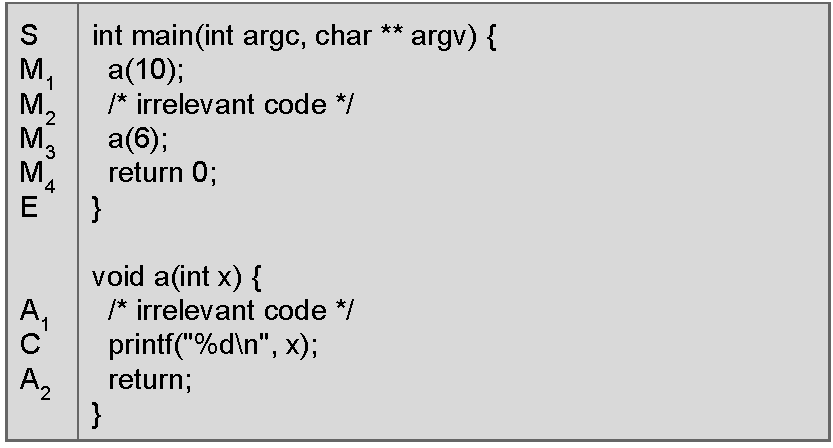
\includegraphics[width=0.6\textwidth]{fig_c4/trace-paths-example.pdf}
	\caption[ScaRR shadow stack example.]{Illustrative example to explain the 
	shadow 
	stack on the ScaRR 
	\emph{Verifier}.}
	\label{fig:trace-paths}
\end{figure}

%We omitted eve5ntually branch instructions in this example. 
In this scenario, an attacker may hijack the return address of the function 
\texttt{a()} in order to jump to the BBL $M_3$.
If this happens, the \emph{Prover} produces the following \emph{online 
measurements}:
$$
(S,C,H_1) \rightarrow (C,C,H_2) \rightarrow (C,C,H_2) \rightarrow \dots.
$$
Although generated after an attack, those measurements are still compliant with 
the checks $(C1)$ and $(C2)$ of the \emph{Verifier}. Thus, to detect this 
attack, we introduce a new relation (\ie \texttt{ret\_to}) to illustrate the 
link between two edges. The \emph{Measurements Generator} computes all the 
\texttt{ret\_to} relations during the \emph{Offline Program Analysis} and saves 
them in the \emph{Measurements DB} using the following notation:
\begin{align*}
(A_2,M_2)~\texttt{ret\_to}~(M_1,A_1), \\
(A_2,M_4)~\texttt{ret\_to}~(M_3,A_1).
\end{align*}

Figure~\ref{fig:shadow-stack} shows how the \emph{Verifier} combines all these 
information to build a remote shadow stack.
%Figure~\ref{fig:shadow-stack-ok} shows a correct sequence of \emph{LoA}s. 
At the beginning, the shadow stack is empty (\ie no function has been invoked 
yet). Then, according to the \emph{online measurement} $(S,C,H_1)$, the 
\emph{Prover} has invoked the \texttt{main()} function passing through the edge 
$(M_1,A_1)$, which is pushed on the top of the stack by the \emph{Verifier}. 
Then, the \emph{online measurement} $(C,C,H_2)$ indicates that the execution 
path exited from the function \emph{a()} through the edge $(A_2,M_2)$, which is 
in relation with the edge on the  top of the stack and therefore is valid.
Moving forward, the \emph{Verifier} pops from the stack and pushes the edge 
$(M_3,A_1)$, which corresponds to the second invocation of the function 
\texttt{a()}.
At this point, the third measurement $(C,C,H_2)$ indicates that the 
\emph{Prover} exited from the function \texttt{a()}
through the edge $(A_2,M_2)$, which is not in relation with $(M_3,A_1)$. Thus, 
the  \emph{Verifier} detects the attack and triggers an alarm. 

\begin{figure}[t]
	\centering
	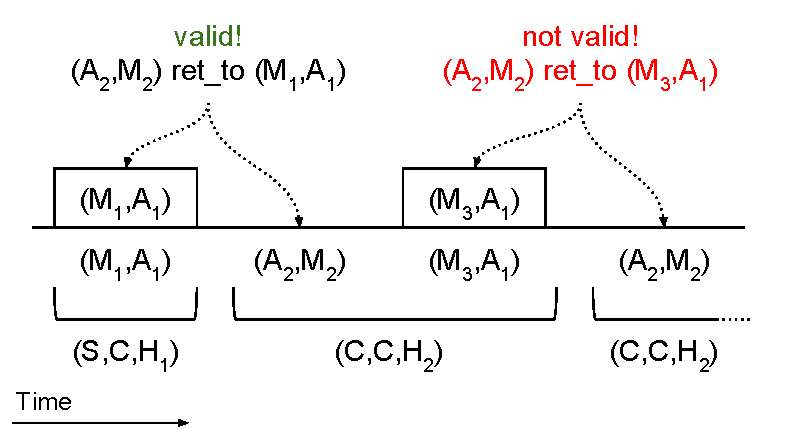
\includegraphics[width=0.6\textwidth]{fig_c4/shadow-stack-no.pdf}
	\caption{Implementation of the shadow stack on the ScaRR \emph{Verifier}.}
	\label{fig:shadow-stack}
\end{figure}

\section{Implementation}
\label{sec:implementation}

Here, we provide the technical details of the ScaRR schema and, in particular, 
of the \emph{Measurements Generator} 
(Section~\ref{ssec:measurements_generator}) and of the \emph{Prover} 
(Section~\ref{ssec:prover}). 

%\subsection{Application CFG (Step 1)} 
\subsection{Measurements Generator}
\label{ssec:measurements_generator}
The \emph{Measurements Generator} is implemented as a compiler, based on 
LLVM~\cite{lattner2004llvm} and on the CRAB framework~\cite{gange2016abstract}. 
Despite this approach, it is also possible to use frameworks to lift the binary 
code to LLVM intermediate-representation (IR)~\cite{mcsema}.

The \emph{Measurements Generator} requires the program source code to perform 
the following operations:
\begin{enumerate*}[label=(\roman*)]
	\item generating the \emph{offline measurements}, and 
	\item detecting and instrumenting the control-flow events.
\end{enumerate*}
During the compilation, the \emph{Measurements Generator} analyzes the LLVM IR 
to identify the control-flow events and generate the \emph{offline 
measurements}, while it uses the CRAB LLVM framework to generate the CFG, since 
it provides a heap abstract domain that resolves indirect forward jumps.
Again during the compilation, the \emph{Measurements Generator} instruments 
each control-flow event to invoke a tracing function 
which is contained in the trusted anchor.
To map LLVM IR BBLs to assembly BBLs, we remove the optimization flags and we 
include dummy code,
which is removed after the compilation through a binary-rewriting tool.
%The updates on the LLVM, that enable the analysis and instrumentation, require 
To provide the above-mentioned functionalities, we add around $3.5$K lines of 
code on top of CRAB and LLVM $5.0$.

\subsection{Prover}
\label{ssec:prover}
The \emph{Prover} is responsible for running the monitored application, 
generating the application \emph{online measurements} and sending the partial 
reports to the \emph{Verifier}. 
To achieve the second aim, the \emph{Prover} relies on the architecture 
depicted in Figure~\ref{fig:architecture_scarr}, which encompasses several 
components 
belonging either to the user-space (\ie \emph{Application Process} and 
\emph{ScaRR Libraries}) or to the kernel-space (\ie \emph{ScaRR 
sys\_addaction}, \emph{ScaRR Module}, and \emph{ScaRR sys\_measure}). 

Each component works as follows:  
\begin{itemize}
	\item \emph{Application Process} - the process running the monitored 
	application, which is equipped with the required instrumentation for 
	detecting control-flow events at runtime.
	\item \emph{ScaRR Libraries} - the libraries added to the original 
	application to trace control-flow events and \emph{checkpoints}.
	\item \emph{ScaRR sys\_addaction} - a custom kernel syscall used to trace 
	control-flow events.
	\item \emph{ScaRR Module} - a module that keeps trace of the \emph{online 
	measurements} and of the partial reports. It also extracts the BBL labels 
	from their runtime addresses, since the ASLR protection changes the BBLs 
	location at each run.
	\item \emph{ScaRR sys\_measure} - a custom kernel syscall used to generate 
	the \emph{online measurements}. 
\end{itemize}
When the \emph{Prover} receives a challenge, it starts the execution of the 
application and creates a new \emph{online measurement}.
During the execution, the application can encounter \emph{checkpoints} or 
control-flow events, both hooked by the instrumentation.
Every time the application crosses a control-flow event, the \emph{ScaRR 
Libraries}
invoke the \emph{ScaRR sys\_addaction} syscall to save the new edge in a buffer 
inside the kernel-space.
While, every time the application crosses a \emph{checkpoint}, the \emph{ScaRR 
Libraries}
invoke the \emph{ScaRR sys\_measure} syscall to save the \emph{checkpoint}
in the current \emph{online measurement}, calculate the hash of the edges saved 
so far, and,
finally, store the \emph{online measurement} in a buffer located in the 
kernel-space.
When the predefined number of \emph{online measurements} is reached, 
the \emph{Prover} sends a partial report to the \emph{Verifier} and starts 
collecting new \emph{online measurements}.
The \emph{Prover} sends the partial report by using a dedicated kernel thread.
The whole procedure is repeated until the application finishes processing the 
input of the \emph{Verifier}. 

The whole architecture of the \emph{Prover} relies on the kernel as a trusted 
anchor, since we find it more efficient in comparison to other commercial 
trusted platforms, such as SGX and TrustZone, but other approaches can be also 
considered (Section~\ref{sec:discussion}). To develop the kernel side of the 
architecture, we add around $200$ lines of code to a Kernel version 
v$4.17$-rc$3$.
We also include the Blake2 source~\cite{Aumasson2014,blake2}, which is faster 
and provides high cryptographic security guarantees for calculating the hash of 
the \emph{LoAs}.
\begin{figure}[t]
	\centering
	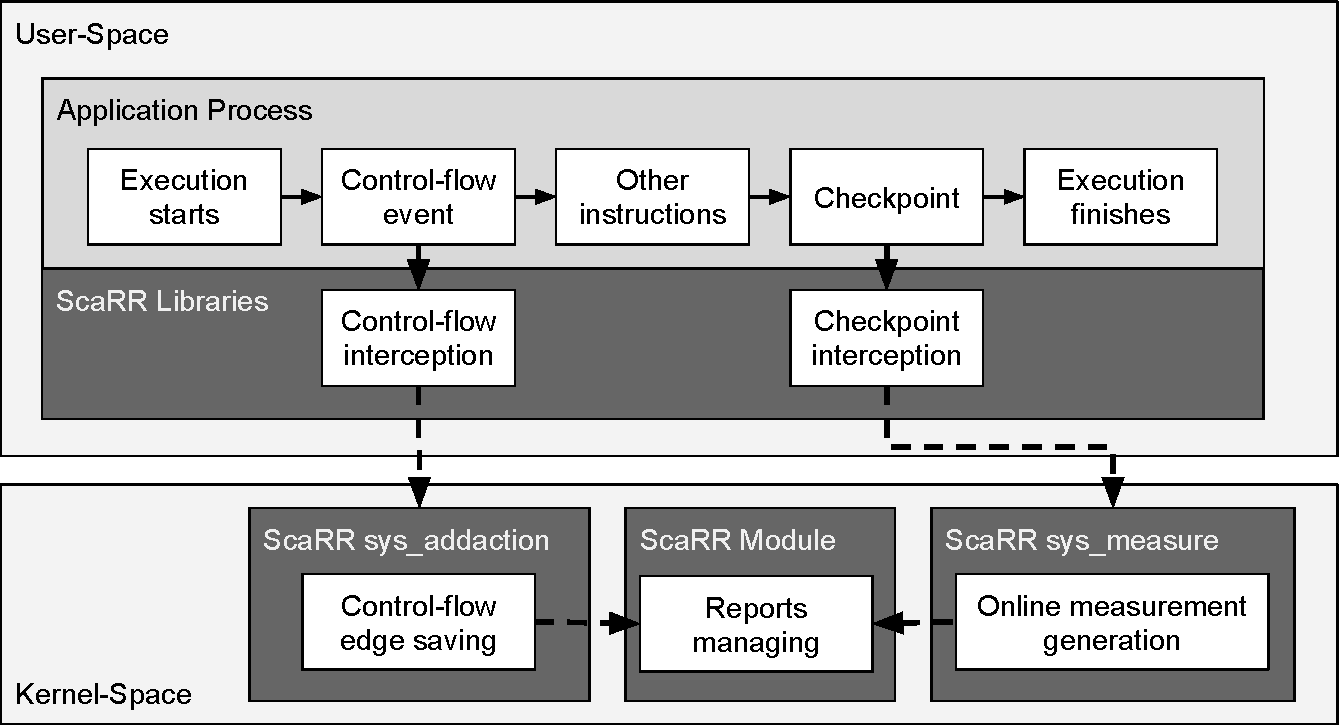
\includegraphics[width=0.7\textwidth]{fig_c4/architecture.pdf}
	\caption{Internal architecture of the \emph{Prover}.}
	\label{fig:architecture_scarr}
\end{figure}

\section{Evaluation}
\label{sec:evaluation}
We evaluate ScaRR from two perspectives.
First, we measure its performance focusing on: attestation speed 
(Section~\ref{ssec:attestation-speed}), verification speed 
(Section~\ref{ssec:verification-speed}) and network impact 
(Section~\ref{ssec:network-impact}).
Then, we discuss ScaRR security guarantees 
(Section~\ref{ssec:security+privacy+consideration}). 

We obtained the results described in this section by running the bench-marking 
suite SPEC CPU 2017 over a Linux machine
equipped with an Intel i7 processor and 16GB of memory~\footnote{We did not 
manage to map assembly BBL addresses to LLVM IR for 519.lbm\_r and 
520.omnetpp\_r.}.
We instrumented each tool to detect all the necessary control-flow events, we 
then extracted the \emph{offline measurements} and we ran each experiment to 
analyze a specific performance metrics. 

\subsection{Attestation Speed}
\label{ssec:attestation-speed}
We measure the attestation speed as the number of \emph{online measurements} 
per second generated by the \emph{Prover}. 
Figure~\ref{fig:attesetation_speed} shows the average attestation speed and the 
standard deviation for each experiment of the SPEC CPU 2017. 
More specifically, we run each experiment 10 times, calculate the number of 
\emph{online measurements} generated per second in each run, and we compute the 
final average and standard deviation. 
Our results show that ScaRR has a range of attestation speed which goes from 
$250$K (510.parest) to over $400$K (505.mcf) of \emph{online measurements} per 
second. This variability in performance depends on the complexity of the single 
experiment and on other issues, such as the file loading. Previous works prove 
to have an attestation speed around $20K$/ $30K$ of control-flow events per 
second~\cite{aberadiat,abera2016c}. Since each \emph{online measurement} 
contains at least a control-flow event, we can claim that ScaRR has an 
attestation speed at least $10$ times faster than the one offered by the 
existing solutions.


\subsection{Verification Speed}
\label{ssec:verification-speed}
During the validation of the partial reports, the \emph{Verifier} performs a 
lookup against the \emph{Measurements DB} and an update of the shadow stack. 
To evaluate the overall performance of the \emph{Verifier}, we consider the 
verification speed as the maximum number of \emph{online measurements} verified 
per second. 
To measure this metrics, we perform the following experiment for each SPEC tool:
first, we use the \emph{Prover} to generate and save the \emph{online 
measurements} of a SPEC tool; 
then, the \emph{Verifier} verifies all of them without involving any element 
that might introduce delay (\eg network). 
In addition, we also introduce a digital fingerprint based on 
AES~\cite{Stallings:2002:AES:763194.763196} to simulate an ideal scenario in 
which the \emph{Prover} is fast. 
We perform the verification by loading the \emph{offline measurements} in an 
in-memory hash map and performing the shadow stack.
Finally, we compute the average verification speed of all tools.

According to our experiments, the average verification speed is 2M of 
\emph{online measurements} per second, with a range that goes from $1.4$M to 
$2.7$M of \emph{online measurements} per second. This result outperforms 
previous works in which the authors reported a verification speed that goes 
from $110$~\cite{Dessouky:2018:LLH:3240765.3240821} to $30$K~\cite{aberadiat} 
of control-flow events per second. As for the attestation speed, we recall that 
each \emph{online measurement} contains at least one control-flow event.

The performance of the shadow stack depends on the number of 
procedure calls and procedure returns found during the generation of 
\emph{online measurements} in the \emph{Online Program Analysis} phase. 
To estimate the impact on the shadow stack, we run each experiment of the SPEC 
CPU 2017 tool and count the number of procedure calls and procedure returns. 
Figure~\ref{fig:functioncall} shows the average number of the above-mentioned 
variables found for each experiment. 
\begin{figure}[t]
	\centering
	\begin{subfigure}[t]{0.45\textwidth}
		\centering
		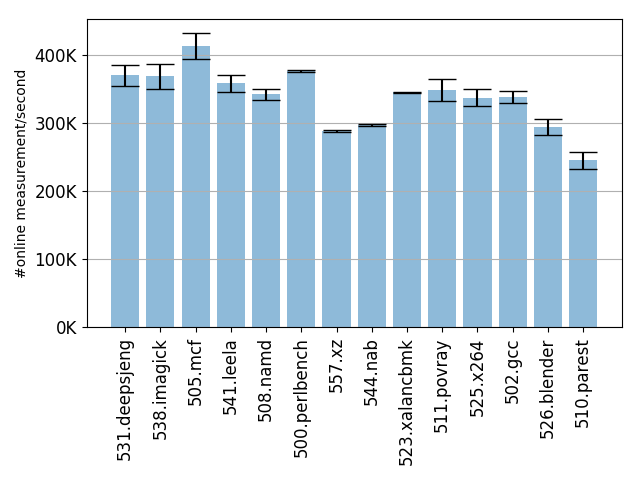
\includegraphics[width=\textwidth]{fig_c4/attesetation_speed.png}
		\caption{Average attestation speed measured as number of online 
			measurements per second.}
		\label{fig:attesetation_speed}
	\end{subfigure} 
	\hfill
	\begin{subfigure}[t]{0.45\textwidth}
		\centering
		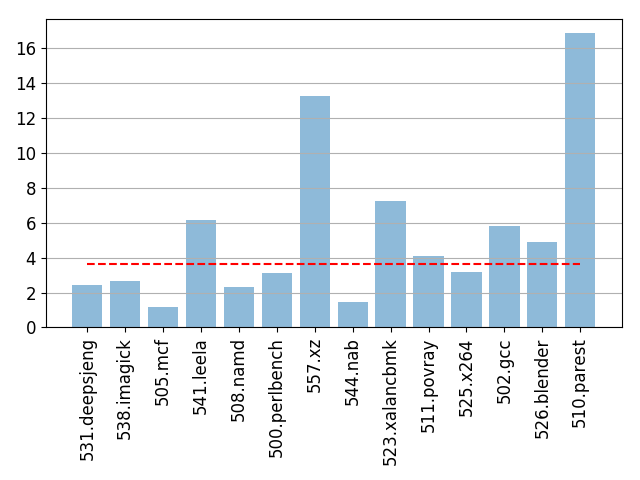
\includegraphics[width=\textwidth]{fig_c4/functioncall.png}
		\caption{Average number of procedure calls and procedure returns found 
		during the \emph{Online Program Analysis} of the SPEC CPU 2017 tools.}
		\label{fig:functioncall}
	\end{subfigure}
	\caption[ScaRR evaluation.]{ScaRR evaluation of attestation speed, and 
	number the procedures invoked.}
	\label{fig:scarr_evaluation}
\end{figure} 
For some experiments (\ie 505.mcf and 544.nab), the average number is almost 
one since they include some recursive algorithms that correspond to small 
\emph{LoAs}. If the average length of the \emph{LoA}s tends to one, ScaRR 
behaves similarly to other remote RA solutions that are based on cumulative 
hashes~\cite{abera2016c,aberadiat}. Overall, Figure~\ref{fig:functioncall} 
shows that a median of push/pop operations is less than $4$, which implies a 
fast update.
Combining an in-memory hash map and a shadow stack allows ScaRR to perform a 
fast verification phase.


%\subsection{Network Impact and Mitigation (Step 4 and Step 5)}
\subsection{Network Impact and Mitigation}
\label{ssec:network-impact}
A high sending rate of partial reports from the \emph{Prover}
might generate a network congestion and therefore affect the verification phase.
To reduce network congestion and improve verification speed, we perform an 
empirical measurement of 
the amount of data (\ie MB) sent on a local network with respect to the 
verification speed by applying different settings.
The experiment setup is similar to Section~\ref{ssec:verification-speed}, but 
the \emph{Prover} and the \emph{Verifier} are connected through an Ethernet 
network with a bandwidth of $10$Mbit/s.
At first, we record $1$M of \emph{online measurements} for each SPEC CPU 2017 
tool.
Then, we send the partial reports to the \emph{Verifier} over a TCP connection,
each time adopting a different approach among the following ones:
\emph{Single}, \emph{Batch}, \emph{Zip}~\cite{zip}, \emph{Lzma}~\cite{lzma}, 
\emph{Bz2}~\cite{bz2} and \emph{ZStandard}~\cite{zstandard}. 
The results of this experiment are shown in 
Figure~\ref{fig:network_performance}. 
In the first two modes (\ie \emph{Single} and  \emph{Batch}),
we send a single \emph{online measurement} and $50$K
\emph{online measurements} in each partial report, respectively.
As shown in the graph, both approaches generate a high amount of network 
traffic (around $80$MB),
introducing a network delay which slows down the verification speed.
For the other four approaches, each partial report still contains $50$K 
\emph{online measurements},
but it is generated through different compression algorithms.
All the four algorithms provide a high compression rate (on average over 
$95$\%) with a consequent reduction in the network overload.
However, the algorithms have also different compression and decompression 
delays, which affect the verification speed.
The \emph{Zip} and \emph{ZStandard} show the best performances with $1.2$M of 
\emph{online measurements}/s and $1.6$M of \emph{online measurements}/s, 
respectively, while \emph{Bz2} ($30$K of online measurements/s) and \emph{Lzma} 
($0.4$M of online measurements/s) are the worst ones. 
The number of \emph{online measurements} per partial report might introduce a 
delay in
detecting attacks and its value depends on the monitored application.
We opted for $50$K because the SPEC CPU tools generate a high number of 
\emph{online measurements} overall.
However, this parameter strictly depends on the monitored application.
This experiment shows that we can use compression algorithms to mitigate the 
network congestion and keep a high verification speed.

\begin{figure}[t]
	\centering
	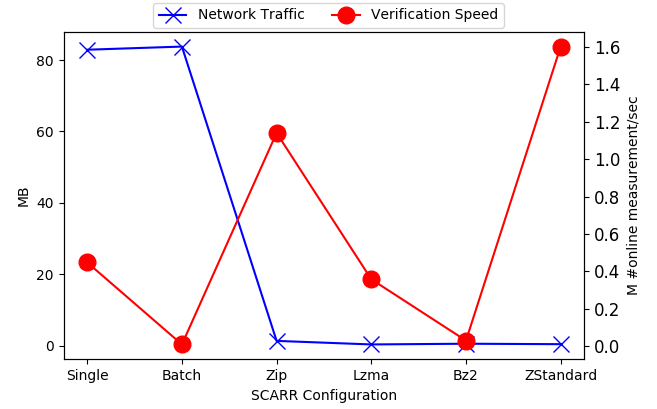
\includegraphics[width=0.5\textwidth]{fig_c4/network_performance.png}
	\caption[ScaRR network traffic evaluation.]{Comparison of different 
	approaches for generating partial repors in terms of network traffic and 
	verification speed.}
	\label{fig:network_performance}
\end{figure} 

\subsection{Attack Detection}
\label{ssec:security+privacy+consideration}
Here, we describe the security guarantees introduced by ScaRR. 

\textbf{Code Injection.}
In this scenario, an attacker loads malicious code, \eg \emph{Shellcode}, into 
memory and executes it by exploiting a memory corruption 
error~\cite{smith1997stack}.
A typical approach is to inject code into a buffer which is under the attacker 
control.
The adversary can, then, exploit vulnerabilities (\eg buffer overflows) to 
hijack the program control-flow towards the shellcode (\eg by corrupting a 
function return address).

When a W$\oplus$X protection is in place, this attempt will generate a memory 
protection error, since the injected code is placed in a writable memory area 
and it is not executable. In case there is no W$\oplus$X enabled, the attack 
will generate a wrong \emph{LoA} detected by the \emph{Verifier}.

Another strategy might be to overwrite a node (\ie a BBL) already present in 
memory. 
Even though this attempt is mitigated by W$\oplus$X, as executable memory 
regions are not writable, it is still possible to perform the attack by 
changing the memory protection attributes through the operating system 
interface (\eg the \texttt{mprotect} system call in Linux), which makes the 
memory area writable. 
The final result would be an override of the application code. Thus, the static 
RA of ScaRR can spot the attack.

\textbf{Return-oriented Programming.}
Compared to previous attacks, the code-reuse ones are more challenging since 
they do not inject new nodes, but they simply reorder legitimate BBLs. Among 
those, the most popular attack~\cite{shacham2007geometry} is 
ROP~\cite{carlini2014rop}, which
exploits small sequences of code (gadgets) that end with a \texttt{ret} 
instruction. Those gadgets already exist in the programs or libraries code, 
therefore, no code is injected. The ROP attacks are Turing-complete in 
nontrivial programs~\cite{carlini2014rop}, and common defence mechanisms are 
still not strong enough to definitely stop this threat.

To perform a ROP attack, an adversary has to link together a set of gadgets 
through the so-called ROP chain, which is a list of gadget addresses. A ROP 
chain is typically injected through a stack overflow vulnerability, by writing 
the chain so that the first gadget address overlaps a function return address. 
Once the function returns, the ROP chain will be triggered and will execute the 
gadget in sequence. Through more advanced techniques such as stack 
pivoting~\cite{PracticalROP}, ROP can also be applied to other classes of 
vulnerabilities, \eg heap corruption.
Intuitively, a ROP attack produces a lot of new edges to concatenate all the 
gadgets, which means invalid \emph{online measurements} that will be detected 
by ScaRR at the first \emph{checkpoint}. 

\textbf{Jump-oriented Programming.}
An alternative to ROP attacks are the JOP 
ones~\cite{yao2013jop,bletsch2011jump}, which exploit special gadgets based on 
indirect \texttt{jump} and \texttt{call} instructions.
ScaRR can detect those attacks since they deviate from the original 
control-flow.

\textbf{Function Reuse Attacks.}
Those attacks rely on a sequence of subroutines, that are called in an 
unexpected order, \eg through virtual functions calls in C++ objects. ScaRR can 
detect these attacks, since the ScaRR control-flow model considers both the 
calling and the target addresses for each procedure call. Thus, an unexpected 
invocation will result in a wrong \emph{LoA}.
For instance, in Counterfeit Object-Oriented Programming (COOP) 
attacks~\cite{schuster2015counterfeit}, an attacker uses a loop to invoke a set 
of functions by overwriting a \emph{vtable} and invoking functions from 
different calling addresses generates unexpected \emph{LoAs}.

\section{Discussion}
\label{sec:discussion}
In this section we discuss limitations and possible solutions for ScaRR.

\textbf{Control-flow graph.}
Extracting a complete and correct CFG through static analysis is challenging.
While using CRAB as abstract domain framework, we experienced some problems
to infer the correct forward destinations in case of virtual functions. Thus, 
we will investigate new techniques to mitigate this limitation.

\textbf{Reducing context-switch overhead.}
%\todo{add discussion on process trace.}
ScaRR relies on a continuous context-switch between user-space and kernel-space.
As a first attempt, we evaluated SGX as a trusted platform, but we found out 
that the overhead was even higher due to SGX clearing the Translation-Lookaside 
Buffer (TLB)~\cite{stravers2013translation} at each enclave exit.
This caused frequent page walks after each enclave call.
A similar problem was related to the Page-Table Isolation 
(PTI)~\cite{watson2018capability} mechanism in the Linux kernel, which protects 
against the Meltdown vulnerability. 
With PTI enabled, TLB is partially flushed at every context switch, 
significantly increasing the overhead of syscalls.
New trusted platforms have been designed to overcome this problem, but, since 
they mainly address embedded software, they are not suitable for our purpose.
We also investigated technologies such as Intel 
PT~\cite{Ge:2017:GGC:3037697.3037716} to trace 
control-flow events at hardware level, but this would have bound ScaRR to a 
specific proprietary technology and we also found that previous 
works~\cite{Ge:2017:GGC:3037697.3037716,Hu:2018:EUC:3243734.3243797} 
experienced information loss.

\textbf{Physical attacks.}
Physical attacks are aimed at diverting normal control-flow such that the 
program is compromised, but the computed measurements are still valid. Trusted 
computing and RA usually provide protection against physical attacks. In our 
work, we mainly focus on runtime exploitation, considering that ScaRR is 
designed for a deployment on virtual machines. Therefore, we assume to have an 
adversary performing an attack from a remote location or from the user-space 
and the hosts not being able to be physically compromised. As a future work, we 
will investigate new solutions to prevent physical attacks.

\textbf{Data-flow attestation.}
ScaRR is designed to perform runtime RA over a program CFG. Pure data-oriented 
attacks might force the program to execute valid, but undesired paths without 
injecting new edges. To improve our solution, we will investigate possible 
strategies to mitigate this type of attacks, considering the availability of 
recent tools able to automatically run this kind of exploit~\cite{hu2016data}. 

\textbf{Toward a full semantic RA.}
We will investigate new approaches to validate series of \emph{online 
measurements} by using runtime abstract 
interpretation~\cite{Ge:2017:GGC:3037697.3037716,Hu:2018:EUC:3243734.3243797,Liu:2018:RED:3243734.3243826}.
